\section{Resultados y análisis}\label{sec:6_resultados}

A continuación expondremos los resultados que hemos obtenido al aplicar los criterios de selección de candidatos a SLGs sobre las regiones seleccionadas.

\subsection{Candidatos según Negrello et al. y González-Nuevo et al. }\label{subsec:resultados_criterios_anteriores}

Nosotros hemos utilizado los criterios de \cite{article:Negrello_2010} y de \cite{article:Nuevo_2012} para identificar SLGs en el catálogo \hatlas\ DR1 y hemos encontrado que hay 20 objetos que cumplen el criterio de \cite{article:Negrello_2010}, 147 que cumplen el criterio de \cite{article:Nuevo_2012} y 10 que cumplen ambos criterios. Teniendo en cuenta que el catálogo cubre un área de \maths{\sim 161\:\mathrm{deg}^2} estimamos que hay una densidad de objetos de \maths{\sim 0.124\:\mathrm{deg}^{-2}} para aquellos que cumplen el primer criterio, de \maths{\sim 0.913\:\mathrm{deg}^{-2}} que cumplen el segundo y de \maths{\sim 0.975\:\mathrm{deg}^{-2}} si consideramos todos aquellos objetos que cumplen al menos uno de los criterios anteriores. 

Por tanto las densidades de objetos que cumplen estos criterios en el catálogo \hatlas\ DR1 son inferiores a las estimaciones previas que se habían realizado. Compárese la densidad de objetos que hemos encontrado, \maths{\sim0.1\:\mathrm{deg}^{-2}} y  \maths{\sim1\:\mathrm{deg}^{-2}} cuando las estimaciones eran \maths{\sim 0.3\:\mathrm{deg}^{-2}} y \maths{\sim 1.5-2\:\mathrm{deg}^{-2}} respectivamente \citep{article:Nuevo_2012}.

\subsection{Candidatos según el criterio bayesiano}\label{subsec:6_slgs_propuestos}

En la zona de intersección de los catálogos \hatlas\ DR1 y \gama\  se han encontrado 3824 contrapartidas que cumplen las condiciones para ser candidatos a sistema lente gravitatoria según el criterio bayesiano que hemos propuesto en la Sección~\ref{sec:5_halos}. Este conjunto contrapartidas se ha dividido en dos categorías. La primera formada por aquellas observaciones que disponían de \rt\ espectroscópico en ambos casos y la segunda formada por las observaciones pertenecientes al catálogo \hatlas\ que tienen un \rt\ obtenido mediante el procedimiento descrito en la Sección~\ref{sec:3_redshift_hatlas}. De la primera categoría se han encontrado 116 contrapartidas y de la segunda 3708. Entre las contrapartidas propuestos se han encontrado 16 en las cuales la observación de \hatlas\ cumple los criterios de \cite{article:Nuevo_2012} o \cite{article:Negrello_2010} para ser SLGs. 

Por otra parte también se ha realizado una simulación en la que a cada observación se le ha reasignado una posición aleatoria sobre una región con un área equivalente al área del catálogo al que pertenece. Después estas dos regiones se han solapado en un área igual al área de intersección de los catálogos originales y se ha procedido ha realizar un conteo de las contrapartidas exactamente de la misma forma que la que se ha llevado a cabo con las muestras originales. Esta simulación se ha repetido mil veces encontrándose \maths{3521\pm58} contrapartidas que cumplen los criterios para ser candidatas a sistema lente gravitatoria, de las cuales \maths{111\pm11} pertenecen a la primera categoría y \maths{3410\pm57} pertenecen a la segunda. Entre estos candidatos hay \maths{26\pm5} contrapartidas en las que además la observación en \hatlas\ cumple los criterios de \cite{article:Nuevo_2012} o \cite{article:Negrello_2010}.

Estos resultados indican que hay \maths{\sim200-300} contrapartidas que no pueden ser explicadas por una distribución aleatoria de las observaciones, sin embargo, evidencian también que nuestra muestra tiene un número muy elevado de contrapartidas formadas por observaciones que no tienen ninguna relación entre sí. 

La mayor diferencia entre la muestra simulada y la real se encuentra entre los objetos de la segunda categoría con una diferencia de un \maths{8\%} de la muestra real. También es significativo que en la muestra simulada se estén encontrando más contrapartidas en las que se cumplen los criterios de \cite{article:Nuevo_2012} o \cite{article:Negrello_2010} que para el caso de la muestra real. Esto nos está indicando que los objetos seleccionados por nuestro criterio de identificación\linebreak son diferentes a los seleccionados por estos dos criterios para la identificación de SLGs.

\begin{figure}[ht]
\captionsetup[subfigure]{labelformat=empty}
  \begin{center} 
  
    \subfloat[]{
     \label{subfig:log_bayes_ajuste}
      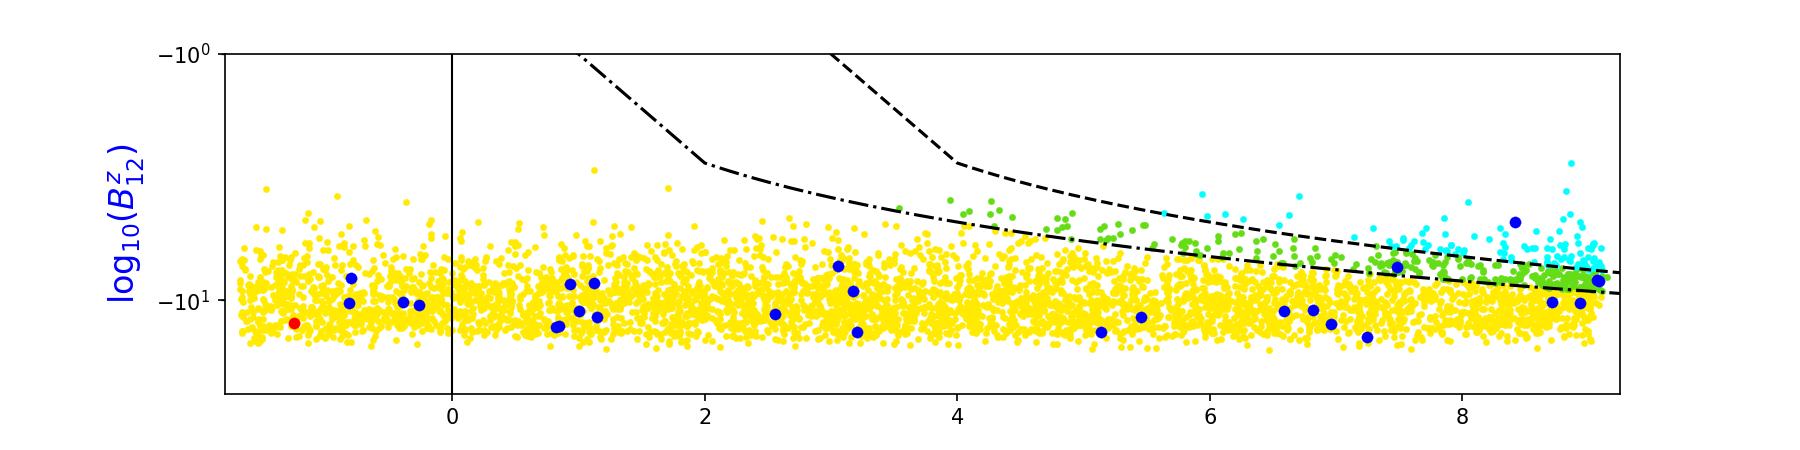
\includegraphics[width=\textwidth]{6_Resultados/matching_ghfactor_bayes_log_semilog_ajuste.png}}
      \vspace*{-23mm}
      
    \subfloat[]{
     \label{subfig:log_bayes_todos}
      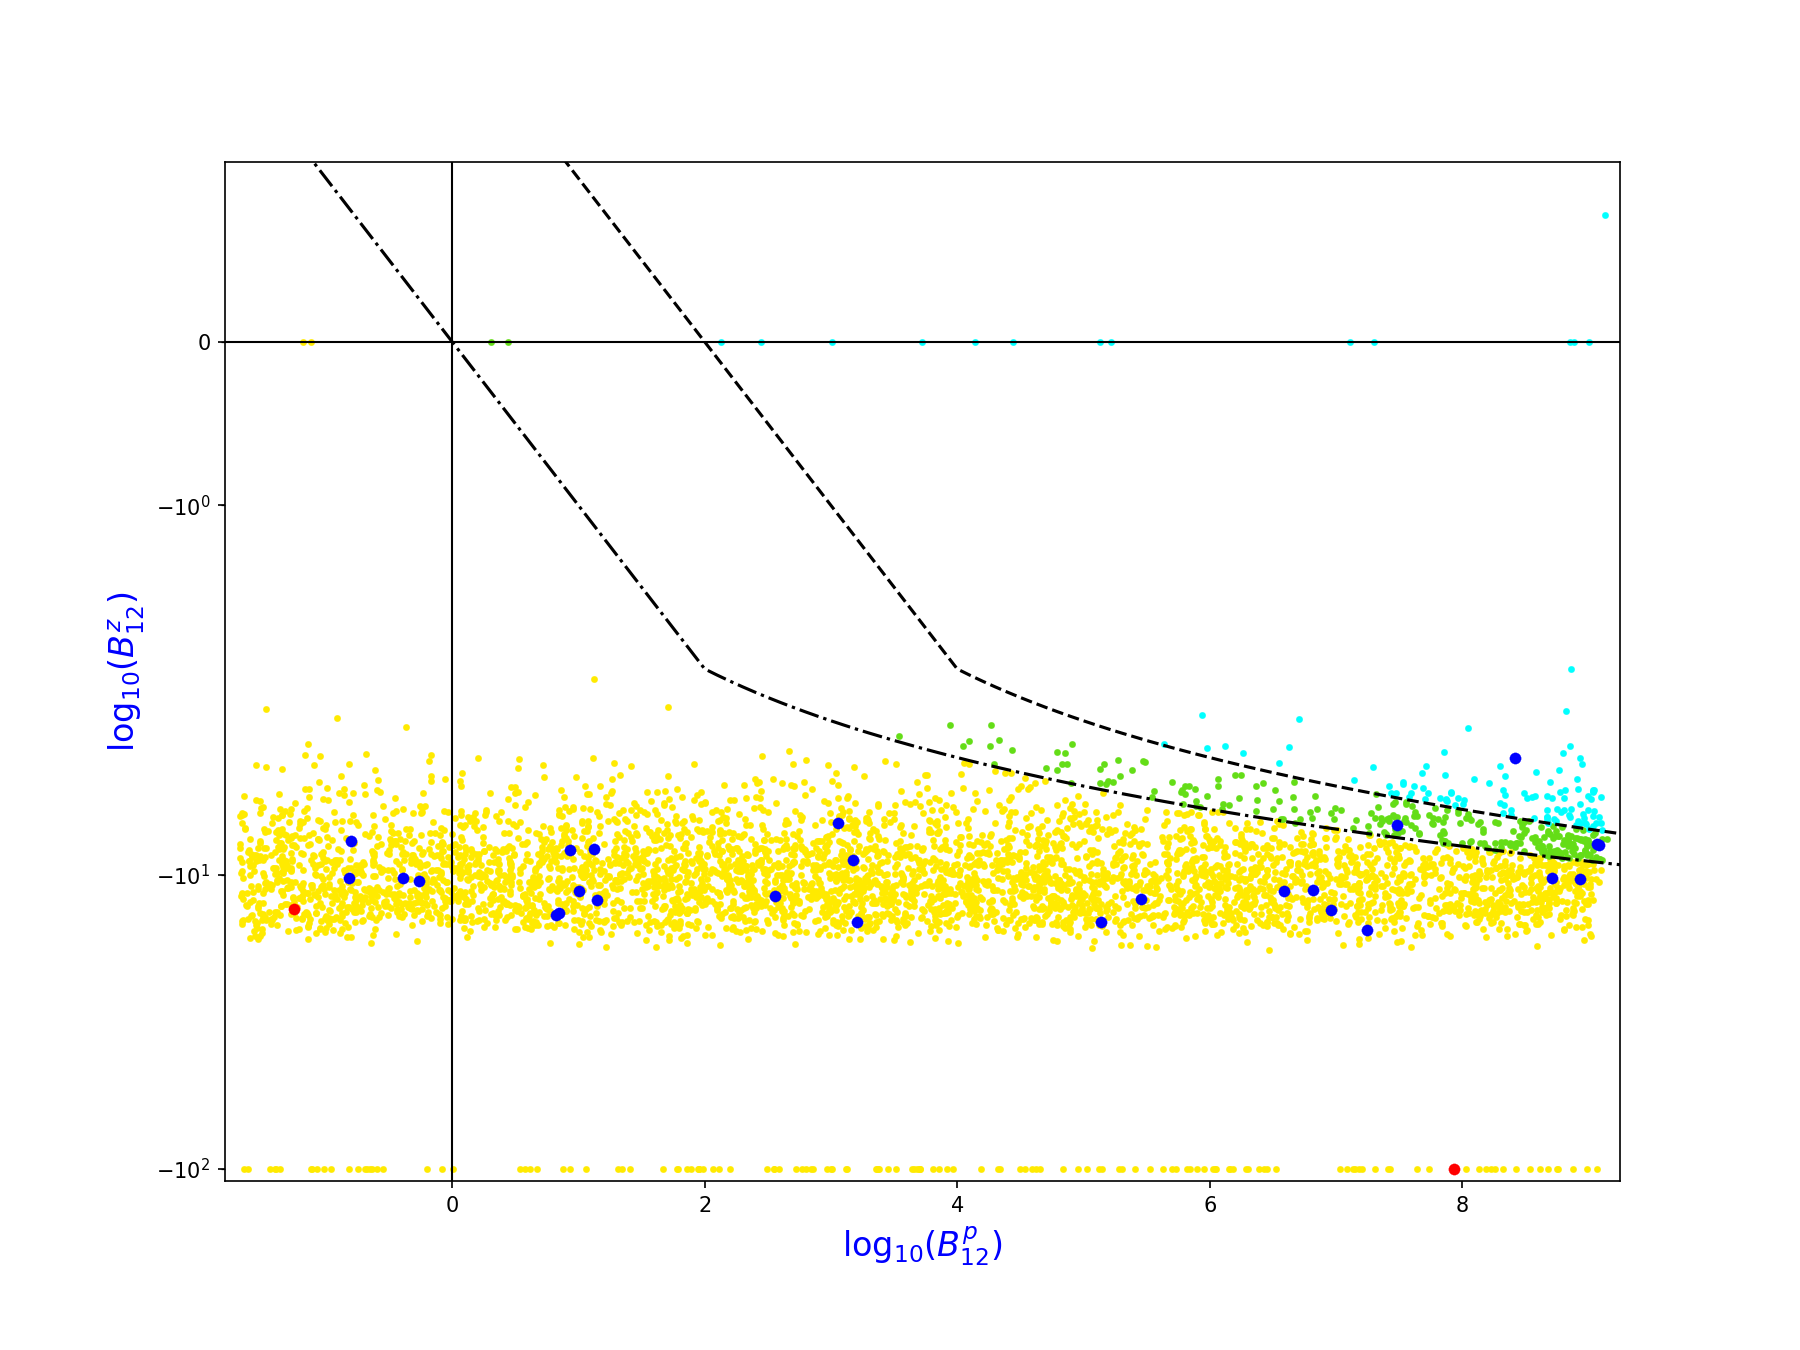
\includegraphics[width=\textwidth]{6_Resultados/matching_ghfactor_bayes_log_semilog.png}}
      
  \end{center}
  \vspace*{-20mm}
  \caption{\small Representación del logaritmo en base diez del factor de Bayes espectroscópico, \maths{B^{z}_{12}} (en la figura, el logaritmo está en escala logarítmica) frente al logaritmo en base diez del factor de Bayes posicional, \maths{B^{p}_{12}} para un total de 4938 emparejamientos que cumplen que \maths{z_{h}\;>\,1}, \maths{z_{h}>z_{g}} y \maths{\phi<54\;\mathrm{arcsec}}. Los puntos de color rojo son los pareados en los que participa un candidato a \halo\ que cumple el criterio de \cite{article:Negrello_2010}; en los de color azul añil participa un candidato a \halo\ que no cumple la condición anterior, pero si que cumple el criterio de \cite{article:Nuevo_2012}; los de color azul cian, son aquellos que no cumplen ninguno de los criterios anteriores pero tienen un  valor \maths{B_{12}>100} (la confianza sobre la hipótesis de que se trata del mismo objeto es absoluta); los de color verde no cumplen ninguno de los criterios anteriores pero \maths{1>B_{12}>100}; el resto de pareados se representan de color anaranjado. Dado que \maths{\log_{10}(0)=-\infty}, cuando se cumple la condición de que el pareado tiene un valor \maths{B^{z}_{12}<{10}^{-100}} entonces se le reasigna el valor  \maths{B^{z}_{12}={10}^{-100}}. La línea vertical continua divide la figura en dos secciones, con \maths{B^{p}_{12}<1} y \maths{B^{p}_{12}>1}. Los puntos con \maths{B^{p}_{12}<1} se corresponden con aquellas contrapartidas con una separación angular \maths{\phi\geqslant49.64\:\mathrm{arcsec}}. En la zona superior de la figura, se han destacado aquellos pareados en los que participan objetos de \hatlas\ cuyo redshift ha sido calculado mediante el método descrito en la Sección~\ref{sec:3_redshift_hatlas}. Los candidatos propuestos por nuestro criterio están representados en la zona con \maths{B^{p}_{12}>1} y \maths{B_{12}<1}.}
  \label{fig:log_bayes}
\end{figure}